---
layout: post
title:  "Accuracy of diagonal mouse paths"
categories: assignment
background: '/img/posts/accuracyMouse/banner.jpg'
published: true
---
\usepackage{graphicx}
\usepackage{amsmath}
During our day-to-day life we constantly use computers. To improve our efficiency, programs should be ergonomically optimized to increase speed when using the program. This can be done by maximising the accuracy of the user when using the program. The accuracy of a user can be measured in the form of the maximum width of the mouse path when using the program. For laptop users, what path angles should be preferred or avoided? So; Do laptop users on average have the same accuracy with a diagonal mouse path compared to a straight mouse path? 

\section*{Methods}
The dataset used for this experiment was a mouse test done by students at the Eindhoven University of Technology. Outliers of the dataset were removed, by only keeping the 99th percentile of the data whilst keeping maximum data. For this experiment, only trackpad users were selected as this is the group where the highest gain in efficiency can be achieved. All paths were either grouped into a ‘Diagonal’ or ‘Straight’ angle types. To compare the means of these groups, a two-sample t-test was used.  

\section*{Hypothesis}
  $$H_0: \mu_{width straight} = \mu_{width diagonal}$$
  $$H_a: \mu_{width straight} > \mu_{width diagonal}$$

\begin{figure}
	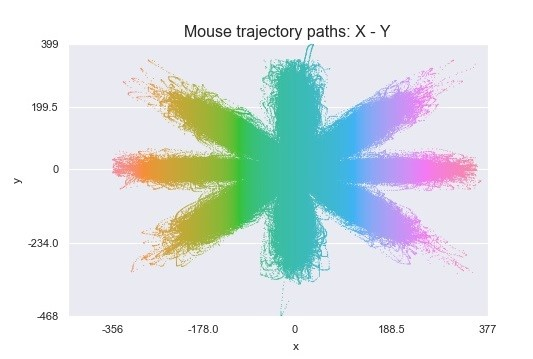
\includegraphics{/img/posts/accuracyMouse/pathsEdited.jpeg}
	\caption{Mouse trajectory paths - all trials}
\end{figure}

% \begin{figure}
% 	\centering
%     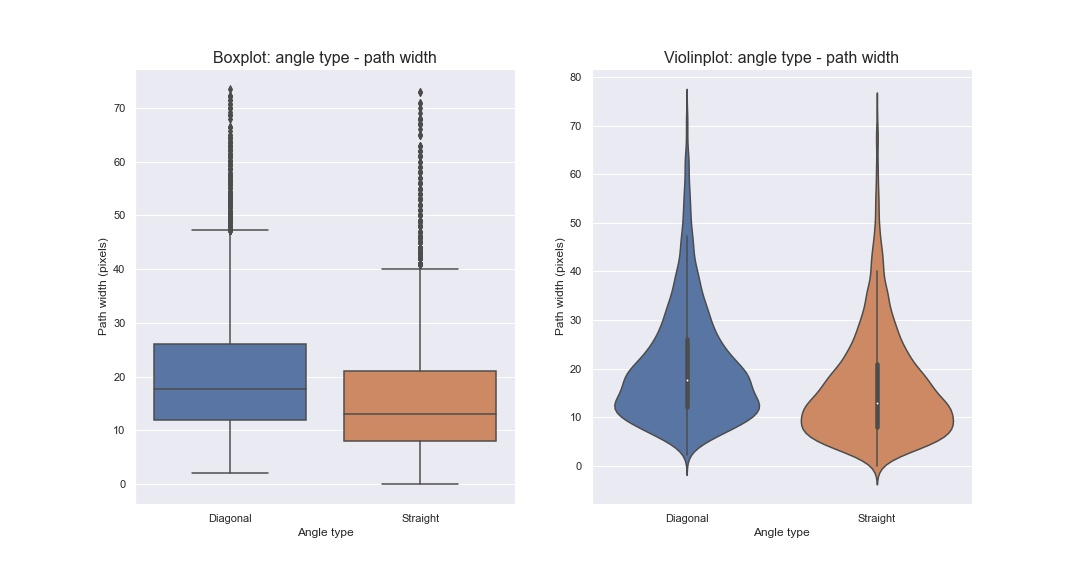
\includegraphics{/img/posts/accuracyMouse/plotAngle.jpeg}
%     \label{fig:angle}
% \end{figure}
\begin{figure}
    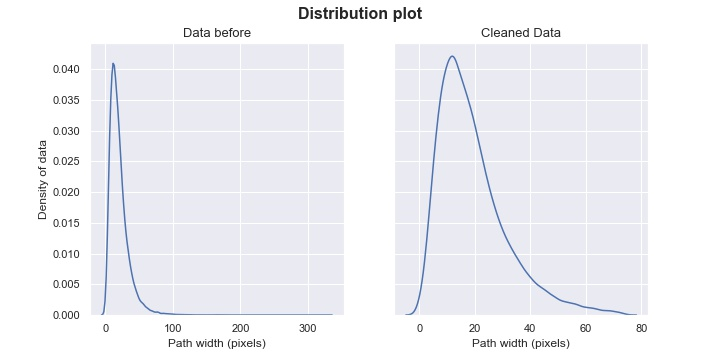
\includegraphics[width=\textwidth]{/img/posts/accuracyMouse/Distribution.jpeg}
    \label{fig:dist}
\end{figure}



\section*{Discussion}
The mouse trajectory paths shows trajectories in all directions, so there are no direction assumptions. The dataset has a length of more than thirteen thousand and is large enough. Even still the length of the dataset is large, the cleaned also follows a distribution curve. For all these reasons, the two-sample t-test is valid and applied. The p-value is (a lot) smaller than an alpha of 0.05, for a 95\% confidence interval. The null hypothesis ($𝐻_0$) is rejected.

\section*{Conclusion}
The null hypothesis ($𝐻_0$) is rejected based on that the p-value is much smaller than an alpha of 0.05, and the alternative hypothesis ($𝐻_𝑎$) is accepted. Meaning, the mean width of trajectories that are straight is lower, and the mean of diagonal trajectories are larger. Trackpad users are less accurate for diagonal trajectories. For using a program, this means that diagonal trajectories should be avoided to aid in maximising accuracy and therefor efficiency. 
